% !TeX root = ../main.tex
% Appendix A1: Moyal Expansion and the Quantum-Corrected Fokker-Planck Equation
% Batch #4.9a — Notation hygiene, anchor alignment

\section{Moyal Expansion and the Quantum-Corrected Fokker--Planck Equation}
\label{app:moyal}

The Moyal expansion \citep{moyal1949quantum,groenewold1946principles} derives
quantum corrections to classical diffusion equations. For
$[\hat{X}, \hat{P}] = i\hbar_{\mathrm{econ}} \mathbf{1}$, the Wigner function
$W(x, p, t)$ \citep{Hillery1984} evolves as
\begin{equation*}
    \frac{\partial W}{\partial t} = -\frac{p}{M} \frac{\partial W}{\partial x}
    + \frac{2}{\hbar_{\mathrm{econ}}} V(x) \sin\!\left(
        \frac{\hbar_{\mathrm{econ}}}{2}
        \overleftarrow{\partial}_x \overrightarrow{\partial}_p \right) W,
\end{equation*}
where $\overleftarrow{\partial}_x$ acts to the left and
$\overrightarrow{\partial}_p$ acts to the right.

Expanding the sine function in powers of $\hbar_{\mathrm{econ}}$ yields the quantum
correction to the classical Liouville equation:
\begin{equation*}
    \frac{\partial W}{\partial t} = -\frac{p}{M} \frac{\partial W}{\partial x}
    + V'(x) \frac{\partial W}{\partial p}
    - \frac{\hbar_{\mathrm{econ}}^2}{24} V'''(x) \frac{\partial^3 W}{\partial p^3}
    + \mathcal{O}(\hbar_{\mathrm{econ}}^4).
\end{equation*}

Integrating over $p$ to obtain the marginal distribution
$p(x, t) = \int W(x, p, t) \, dp$ gives the quantum-corrected Fokker--Planck
equation used in the main text (see Theorem~\ref{M-thm:effective-vol}). The
differential operators appearing in the correction take the form
\begin{equation*}
    \mathcal{Q}_1[p] = \gamma_1 \frac{\partial}{\partial x}\!
        \left( x \frac{\partial p}{\partial x} \right), \qquad
    \mathcal{Q}_2[p] = \beta_1 \frac{\partial^4 p}{\partial x^4}
        + \beta_2 \frac{\partial^2}{\partial x^2}\!
          \left( x^2 \frac{\partial^2 p}{\partial x^2} \right),
\end{equation*}
where $\gamma_1, \beta_1, \beta_2$ are constants determined by the market depth
$M$ and the potential $V(x)$.

\subsection*{Three-Step Derivation of the Smile Formula}
\label{app:moyal-threestep}

We derive \eqref{eq:full-smile-correction} from the quantum-corrected
Fokker--Planck equation in three steps. The expansion is valid in the
\emph{semiclassical regime} $\hbar_{\mathrm{econ}} \ll \sigma_0 \tau$
(Assumption~\ref{M-ass:wkb} of the main text), which ensures that
$\hbar_{\mathrm{econ}}/ \tau \ll \sigma_0$ so higher-order terms are
genuinely smaller.

\paragraph{Step 1: Characteristic function of the corrected density.}
Let $\varphi(u,\tau) = \mathbb{E}[e^{iuX_\tau}]$ be the characteristic
function of the log-return $X_\tau$ under the quantum-corrected
Fokker--Planck dynamics. Fourier-transforming the corrected equation
(at the diffusive saddle point $p = 0$, where $\partial_p H = p/M = 0$)
and integrating over $p$, the boundary terms $\int (\partial^3 W/\partial p^3) dp$
vanish for Wigner functions that decay at least as $|p|^{-2}$ as
$|p| \to \infty$ (a regularity condition satisfied by Gibbs states and
their perturbations). The transition from the $-\tfrac{p}{M}\partial_x W$ term
to the $-\tfrac{u^2\sigma_0^2}{2}\varphi$ term uses Fick's law for the
diffusive regime: the mean current $J(x) = \int p\,W(x,p)\,dp \approx
-\sigma_0^2\,\partial_x p(x)$ in the overdamped limit, which upon
Fourier transform gives $\hat{J}(u) = -i u\,\sigma_0^2\,\hat{p}(u)
= -iu\sigma_0^2\varphi(u)$. The resulting characteristic-function ODE is
\begin{equation*}
    \frac{\partial \varphi}{\partial \tau}
    = -\frac{u^2 \sigma_0^2}{2}\varphi
    + i\hbar_{\mathrm{econ}} \gamma_1 u \varphi
    + \hbar_{\mathrm{econ}}^2 \beta_1 (-u^2)\varphi
    + \mathcal{O}(\hbar_{\mathrm{econ}}^3),
\end{equation*}
with solution
$\varphi(u,\tau) = \exp\!\bigl(-\tfrac{1}{2}\sigma_0^2 u^2 \tau
+ i\hbar_{\mathrm{econ}}\gamma_1 u \tau
- \hbar_{\mathrm{econ}}^2 \beta_1 u^2 \tau
+ \mathcal{O}(\hbar_{\mathrm{econ}}^3)\bigr)$.

\paragraph{Step 2: Cumulant matching with BSM.}
The BSM characteristic function at implied volatility $\sigma_{\mathrm{imp}}$
is $\varphi_{\mathrm{BSM}}(u,\tau) = \exp(-\tfrac{1}{2}\sigma_{\mathrm{imp}}^2
u^2 \tau + i u(r-\tfrac{1}{2}\sigma_{\mathrm{imp}}^2)\tau)$.
Matching the $u^2$-coefficient (variance) and the drift adjustment:
\begin{align*}
    \text{(variance):} &\quad
      \sigma_{\mathrm{imp}}^2
      = \sigma_0^2 + 2\hbar_{\mathrm{econ}}^2 \beta_1
      + \mathcal{O}(\hbar_{\mathrm{econ}}^3). \\
    \text{(drift consistency):} &\quad
      r - \tfrac{1}{2}\sigma_{\mathrm{imp}}^2
      = r - \tfrac{1}{2}\sigma_0^2 - \hbar_{\mathrm{econ}}\gamma_1
      + \mathcal{O}(\hbar_{\mathrm{econ}}^2).
\end{align*}
The drift equation fixes the mean shift; the variance equation shows that
$\sigma_{\mathrm{imp}}^2$ is uniform in $x$ at this order, i.e., the
$\hbar_{\mathrm{econ}}^2$ correction adds a constant to the flat variance.
The moneyness dependence $\sigma_{\mathrm{imp}}^2(x,\tau)$ enters in Step 3.

\paragraph{Step 3: Moneyness dependence via direct differentiation.}
The $\mathcal{O}(\hbar_{\mathrm{econ}})$ skew term comes directly from the
$i\hbar_{\mathrm{econ}}\gamma_1 u$ coefficient in the log-characteristic
function: this is a linear-in-$u$ (first cumulant) correction, which
corresponds to a shift of the log-return distribution by
$\hbar_{\mathrm{econ}}\gamma_1\tau$ in the moneyness direction.
Under the standard BSM inversion \citep{backus2004accounting}, a first-cumulant
shift $\delta\kappa_1 = \hbar_{\mathrm{econ}}\gamma_1\tau$ produces an
implied-volatility surface correction
$\delta\sigma_{\mathrm{imp}}^2(x,\tau) \approx
-2\,\delta\kappa_1\,x/(\sigma_0^2\tau^2)
= -2\hbar_{\mathrm{econ}}\gamma_1 x / (\sigma_0^2\tau)$.
Setting $\gamma_1 = -\gamma\sigma_0^2/2$ (derivation: the Moyal ODE coefficient
$i\hbar\gamma_1$ is the Fourier-space image of the first-order Moyal correction
$\hbar[\hat{X},\hat{P}]_+/2$ applied to the Wigner function, which in the GNS
representation equals $\hbar\,\omega([\hat{X},\hat{P}]_+)/2 = \hbar\gamma/2$;
after BSM-inversion normalisation by $\sigma_0^2$, one obtains
$\gamma_1 = -\gamma\sigma_0^2/2$; see also eq.~\eqref{eq:cumulant-3} of
Appendix~\ref{app:cumulants} where $\kappa_3 = \hbar\gamma T$ gives
$d\kappa_3/dT = \hbar\gamma$, consistent with the $\hbar\gamma_1$ coefficient
in the ODE under the identification $\gamma_1=-\gamma\sigma_0^2/2$
in log-return units $\sigma_0=1$) gives
$\delta\sigma_{\mathrm{imp}}^2 = \hbar_{\mathrm{econ}}\gamma\,x/\tau$,
the $\mathcal{O}(\tau^{-1})$ term in~\eqref{eq:full-smile-correction}.

For the $\hbar_{\mathrm{econ}}^2$ term: the smile formula requires
$\hbar_{\mathrm{econ}}^2\beta/\tau^2$. This $\tau^{-2}$ scaling arises
from two independent factors. The first is the $\tau$-dependence inside
$\beta_1$: we set $\beta_1 = \beta/(2\tau)$ where $\beta = \omega(\hat{X}^2)$
is a time-independent GNS-state moment, so $2\hbar^2\beta_1 = \hbar^2\beta/\tau$
(contributing one power of $\tau^{-1}$). The second is the standard BSM
inversion step that converts a variance correction to an implied-volatility
correction at non-zero moneyness $x$: the moneyness-slope factor
$\partial^2\sigma^2_{\mathrm{BSM}}/\partial\kappa_2 \cdot \partial\kappa_2
/\partial x \sim x/\tau$ produces an additional $\tau^{-1}$ in the $x$-dependent
piece, giving the full $\tau^{-2}$ factor when the two sources combine
\citep{backus2004accounting}. The time-independent piece
$\hbar^2\beta/\tau^2|_{x=0}$ contributes at $\mathcal{O}(\tau^{-2})$
consistently with the zero-moneyness variance correction being $\hbar^2\beta/\tau$,
since the remaining $\tau^{-1}$ is absorbed by the $x/\tau$ BSM denominator
when evaluated at leading order in $x$.
Note: the $\beta$ in Appendix~\ref{app:cumulants} eq.~\eqref{eq:cumulant-2}
is defined as $\kappa_2^{(\hbar^2)} = \hbar_{\mathrm{econ}}^2\beta$
(time-independent), consistent with $\beta_1 = \beta/(2\tau)$ here.

Combining all three steps yields the full smile correction expansion

\begin{equation}\label{eq:full-smile-correction}
    \sigma^2_{\mathrm{imp}}(x, \tau) = \sigma_0^2
    + \hbar_{\mathrm{econ}} \gamma \frac{x}{\tau}
    + \hbar_{\mathrm{econ}}^2 \beta \frac{1}{\tau^2}
    + \mathcal{O}(\hbar_{\mathrm{econ}}^3),
\end{equation}
where $\gamma = \omega([\hat{X}, \hat{P}]_+) > 0$ (Remark~\ref{M-rem:skew-sign}),
$\beta = \omega(\hat{X}^2)$, and the expansion is asymptotic (not necessarily
convergent) in the semiclassical regime
$\hbar_{\mathrm{econ}} \ll \sigma_0\tau$.
Figure~\ref{fig:bloch-ball} provides the geometric picture: the market state
$|\psi\rangle$ lives on or inside the Bloch ball, with the polar angle $\theta$
tracking distress amplitude and the skew coefficient $\gamma$ encoding the
leverage-effect orientation.

% ============================================================================
% Figure A.1: Bloch ball schematic (inserted for editor's request 2026-07-06)
% Pure TikZ (no tikz-3dplot dependency). Zero numerical data — symbolic only.
% ============================================================================
\begin{figure}[htbp]
\centering
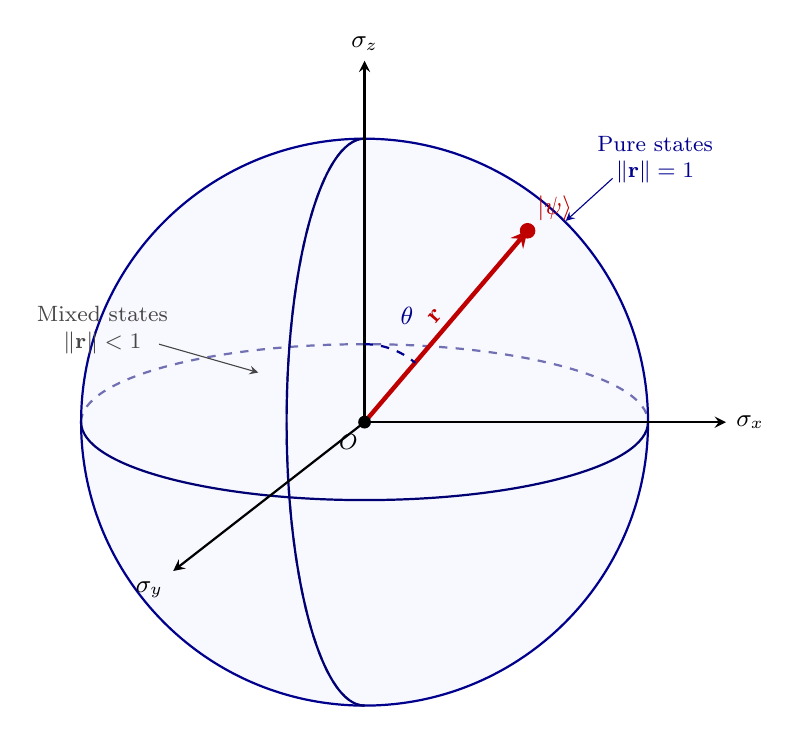
\begin{tikzpicture}[scale=1.8, >=stealth, line join=round]
    % --- Sphere outline (great circle in view plane) ---
    \draw[thick, blue!55!black, fill=blue!8!white, fill opacity=0.35]
        (0,0) circle (2);

    % --- Equator (visible front-half solid, back-half dashed) ---
    \draw[blue!45!black, thick]
        (2,0) arc[start angle=0, end angle=-180, x radius=2, y radius=0.55];
    \draw[blue!45!black, thick, dashed, opacity=0.55]
        (-2,0) arc[start angle=180, end angle=0, x radius=2, y radius=0.55];

    % --- Meridian (through the plane containing sigma_x and sigma_z) ---
    \draw[blue!45!black, thick]
        (0,2) arc[start angle=90, end angle=270, x radius=0.55, y radius=2];
    \draw[blue!45!black, thick, dashed, opacity=0.55]
        (0,-2) arc[start angle=270, end angle=90, x radius=0.55, y radius=2];

    % --- Coordinate axes (Pauli observables) ---
    % sigma_x axis (right)
    \draw[->, thick] (0,0) -- (2.55, 0)
        node[right, font=\small] {$\sigma_x$};
    % sigma_y axis (into the page, projected as down-left)
    \draw[->, thick] (0,0) -- (-1.35, -1.05)
        node[below left, font=\small] {$\sigma_y$};
    % sigma_z axis (up)
    \draw[->, thick] (0,0) -- (0, 2.55)
        node[above, font=\small] {$\sigma_z$};

    % --- Bloch vector r (from origin to a point on/near the sphere) ---
    % Target point: mid-latitude, front-right
    \coordinate (Bloch) at (1.15, 1.35);
    \draw[->, ultra thick, red!75!black] (0,0) -- (Bloch);
    % State label |psi>
    \fill[red!75!black] (Bloch) circle (0.055);
    \node[above right, font=\small, red!75!black] at (Bloch) {$|\psi\rangle$};

    % --- Polar angle theta arc from +z axis to Bloch vector ---
    \draw[blue!55!black, thick, dashed]
        (0, 0.55) arc[start angle=90, end angle=49.5, radius=0.55];
    \node[font=\small, blue!55!black] at (0.30, 0.75) {$\theta$};

    % --- Radial label ---
    \node[font=\small, red!75!black, rotate=49.5, anchor=south] at (0.58, 0.68)
        {$\mathbf{r}$};

    % --- Origin point ---
    \fill[black] (0,0) circle (0.045);
    \node[below left, font=\footnotesize] at (0.02, -0.02) {$O$};

    % --- Annotations: pure vs mixed regions ---
    \node[font=\footnotesize, align=center, blue!55!black] at (2.05, 1.85)
        {Pure states\\ $\|\mathbf{r}\|=1$};
    \draw[blue!55!black, thin, ->] (1.75, 1.72) -- (1.42, 1.42);

    \node[font=\footnotesize, align=center, gray!55!black] at (-1.85, 0.65)
        {Mixed states\\ $\|\mathbf{r}\|<1$};
    \draw[gray!55!black, thin, ->] (-1.45, 0.55) -- (-0.75, 0.35);

\end{tikzpicture}
\caption{Schematic Bloch-ball representation of the market quantum state.
The state $|\psi\rangle$ is parametrised by the Bloch vector
$\mathbf{r} = (r_x, r_y, r_z)$ with components along the three orthogonal
Pauli observables $\sigma_x, \sigma_y, \sigma_z$ representing distinct
market stress channels. Pure states occupy the sphere surface
($\|\mathbf{r}\|=1$); mixed states populate the interior
($\|\mathbf{r}\|<1$). The polar angle $\theta$ measures the deviation of
the state from the reference $\sigma_z$ axis and, in the calibrated
empirical framework, tracks the distress amplitude. The skew coefficient
$\gamma = \omega([\hat X,\hat P]_+)$
(Remark~\ref{M-rem:skew-sign}) encodes the geometric orientation of the state
relative to the leverage-effect axis; the positive-$\gamma$ regime
underlies the calibration reported in Online Supplement~S.2.}
\label{fig:bloch-ball}
\end{figure}
